\subsection{Motor modelling}
A model of a motor consist of both a mechanical and an electrical section, due to the electrical current, $i_a(t)$, conversion into a rotational force called torque, $\tau_m$. Therefore a model of the mechanical and the electrical system is produced. The electrical model provides the motors torque and the mechanical model from the motor provides what contributions the motor delivers to the drivetrain, see \secref{DriveTrain}.

\subsubsection{Electrical model}
The output from the motors electrical model is torque, $\tau_m$. To obtain torque the formula for translating the electrical current, $i_a$, to torque is utilized:

\begin{flalign}\centering
  \tau_m(t) = K_t \cdot i_a(t) %\unit{\volt}
  \label{equ:motortorque}
\end{flalign}
\hspace{6mm} Where:\\
\begin{tabular}{p{1cm}ll}
& $\tau_m$ & the rotational force torque [$N \cdot m$] \\
& $i_a(t)$ & the electrical closed loop current [$A$]\\
& $K_t$ & the torque constant [$\frac{N \cdot m}{A}$] \\
\end{tabular}

An expression for the current, $i_a$, is required to derive a model for the electrical system. In \figref{fig:MotorElectric} an electrical diagram of the motor is display.

\begin{figure}[H]
	\centering
	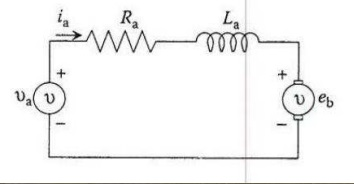
\includegraphics[scale=0.8]{figures/MotorElektrikDiagram.jpg}
	\caption{A electric diagram of the motor}
	\label{fig:MotorElectric}
\end{figure}

By using Kirchoffs voltage law on the closed loop, seen in \figref{fig:MotorElectric}, an expression including $i_a$ can be derived:

\begin{flalign}\centering
V_a(t) = R_a \cdot i_a(t) + L_a \cdot \frac{di_a}{dt} + e_b 
\label{MotorClosedLoop}
\end{flalign}
\hspace{6mm} Where:\\
\begin{tabular}{p{1cm}ll}
& $V_a(t)$ & the supply voltage [$V$] \\
& $R_a$ & the eternal resistance in the motor [$\Omega$]\\
& $L_a$ & the inductance in the motor [$H$] \\
& $e_b$ & the electromotive force, also called EMF [$\V$] \\
\end{tabular}

The electromotive force, $e_b$, is equivalent to:

\begin{flalign}\centering
e_b = K_e \cdot \dot{\theta}_m(t) 
\end{flalign}
\hspace{6mm} Where:\\
\begin{tabular}{p{1cm}ll}
& $K_e$ & the electromotive constant [$Wb$] \\
& $\dot{\theta}_m$ & the angular velocity in the motor [$\frac{rad}{s}$] \\
\end{tabular}

the equivalent for the electromotive force is substituted into \eqref{MotorClosedLoop}.

\begin{flalign}\centering
V_a(t) = R_a \cdot i_a(t) + L_a \cdot \frac{di_a}{dt} + K_e \cdot \dot{\theta}_m(t)
\end{flalign}

The Laplace transform is applied to the derived equation:

\begin{flalign}\centering
V_a(s) = R_a \cdot i_a(s) + L_a \cdot s \cdot i_a(s) + K_e \cdot \dot{\theta}_m(s) 
\end{flalign}

The equation is solved for $i_a$:

\begin{flalign}\centering
i_a(s) = \frac{V_a(s) - K_e \cdot \dot{\theta}_m(s)}{sL_a + R_a} 
\end{flalign}

By substituting the derived equation for $i_a$ into \eqref{equ:motortorque}, a new expression for the motors torque is derived. 

\begin{flalign}\centering
  \tau_m = K_t \cdot i_a(s) = K_t \cdot \frac{V_a(s) - K_e \cdot \dot{\theta}_m(s)}{sL_a + R_a}  %\unit{\volt}
  \label{eq:Totaltorquewithcurrentexpression}
\end{flalign}

A equation for the electrical model relative to the motors torque has been derived.

\subsubsection{Mechanical model}
A mechanical model is formed to analyse the forces and moments affecting the mechanical system, and to see how the system reacts to stimuli.

Newtons second law of motion for rotational systems yields, that torque is equal:

\begin{flalign}\centering
\tau_m(t) = J_m \cdot \ddot{\theta}_m(t)
\label{eq:mechanicalmodel}
\end{flalign}
\hspace{6mm} Where:\\
\begin{tabular}{p{1cm}ll}
& $J_m$ & the motors inertia [$kg*m^2 $] \\
& $\ddot{\theta}_m$ & the angular acceleration in the motor [$\frac{rad}{s^2}$] \\
\end{tabular}

This law is applied to the mechanical model and visualized in \figref{fig:MotorMechanicalModel}. Furthermore it is necessary to consider the friction affecting the rotation of the motor when it is spinning. The friction is the opposite direction of the applied rotational force torque, see \figref{fig:MotorMechanicalModel}.

\begin{figure}[H]
	\centering
	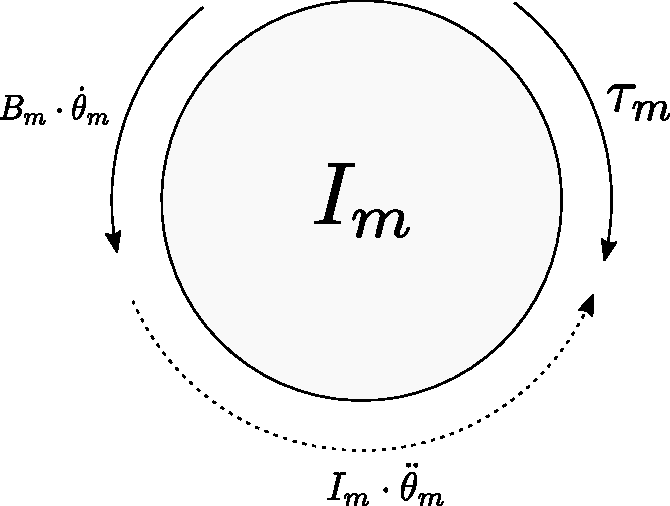
\includegraphics[scale=0.8]{figures/MotorMechanicalModel.pdf}
	\caption{A free body diagram of the motor}
	\label{fig:MotorMechanicalModel}
\end{figure}

From the figure an equation for the mechanical model can be derived.

\begin{flalign}\centering
\tau_m(t) = J_m \cdot \ddot{\theta}_m(t) + B \cdot \dot{\theta}_m(t)
\end{flalign}

The equation is transferred into the frequency domain using the Laplace transform. Furthermore the equation is isolated for the angular velocity enabling a voltage as input an a torque as output: 

\begin{flalign}\centering
\dot{\theta}_m(s) = \frac{\tau_m(s)}{J_m(s) \cdot s+B}
\label{eq:ThetadotforBlock}
\end{flalign}

\eqref{eq:ThetadotforBlock} and \eqref{eq:Totaltorquewithcurrentexpression} delivers the information needed to make a visual representation of the motor model. The input is the supply voltage, $V_a(s)$ delivered to the motor and the output is the required torque, $\tau_m$, see \figref{fig:motormodelBlock}. The block representation of the system can be used, when the system is simulated.

\begin{figure}[H]
	\centering
	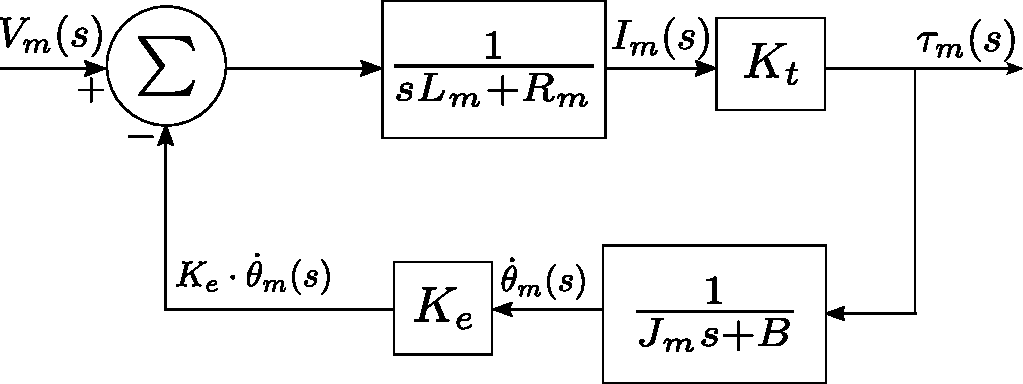
\includegraphics[scale=0.9]{figures/motormodelBlock.pdf}
	\caption{A block representation of the motor, with a voltage, $V_m(s)$, as the input and a rotational force, $\tau_m(s)$, as the output.}
	\label{fig:motormodelBlock}
\end{figure}

A model of the electrical and mechanical part has been formed and combined to a block representation of the motors applied voltage and generated torque. Next step is to model the drivetrain, which connects to the motor through the motor shaft.